\chapter{The Gravitational Field: Waves, Curvature, and the Optical Analogy}
\label{chap:gravitational_field}

Standard General Relativity models gravity as geometric curvature that propagates at the speed of light. Tension Field Theory (TFT) offers a mechanical clarification, distinguishing between the static existence of the Tension Field itself and the dynamic Propagation of Change within that field.

\section{Gravitational Waves: Static Field vs. Dynamic Propagation}

\subsection{The Static Field (Longitudinal Tension)}
The pull of gravity (as defined in \hyperref[chap:restorative_gravity]{Chapter \ref*{chap:restorative_gravity}}) is a tension gradient ($-\nabla\tau$) established in the active Spacetime Gravitational Floor (SGF). Because the latent SGF is hyper-rigid (Postulate I), the existence of the tension field is a state property of the vacuum.

\begin{itemize}
    \item \textbf{Mechanism:} For a static mass (like the Sun), the tension gradient is stable. A planet orbiting it is simply surfing the existing slope of the lattice floor.
    \item \textbf{Result:} This explains why planetary orbits are stable and do not suffer from the retardation aberration that would occur if gravity had to actively ``reach out'' at every moment.
\end{itemize}

\subsection{The Dynamic Wave (Transverse Shear)}
However, when a mass accelerates or changes configuration (for example, a black hole merger), it actively deforms the 3D FCC lattice geometry. This deformation propagates as a macroscopic transverse shear wave.

\begin{itemize}
    \item \textbf{Mechanism:} The isochoric transverse geometric shear of the solid lattice nodes creates a transient structural oscillation in the local FCC architecture without displacing the interstitial condensate.
    \item \textbf{Speed (The 2D/3D Unification):} Because this propagation involves macroscopic bulk structural shear, the wave speed is strictly determined by the ratio of the continuum's 3D Volumetric Shear Stiffness ($K_{\mathrm{shear}}$) to its macroscopic Effective Inertial Density ($\rho_{\mathrm{eff}}$). This yields the exact same absolute elastic speed limit ($c_{\mathrm{E}}$) that governs 2D light propagation:
\end{itemize}

\begin{equation}
    c_{\mathrm{GW}} = \sqrt{\frac{K_{\mathrm{shear}}}{\rho_{\mathrm{eff}}}} \equiv c_{\mathrm{E}}
\end{equation}

\noindent\textbf{Result:} This confirms why Gravitational Waves ($c_{\mathrm{GW}}$) travel at exactly the speed of light ($c_{\mathrm{E}}$). While light is a 2D surface tension ripple and gravity is a 3D volumetric shear wave, both are mechanical oscillations of the exact same hyper-rigid visco-elastic scaffold.

\vspace{0.5em}
\noindent \textbf{Cosmological Redshift (Visco-Elastic Phase Lag):} Because both light and gravitational waves are transverse shear deformations rubbing against the exact same interstitial condensate, they are subjected to the exact same boundary friction ($\Gamma_{\mathrm{D}}$). Therefore, gravitational waves lose energy (redshift) over cosmic distances at the exact same rate as optical light ($H_0 \equiv \Gamma_{\mathrm{D}}$). This perfectly aligns with LIGO's observational requirement to correct for the cosmological redshift of gravitational waves; the wave is not being stretched by expanding space, it is simply bleeding energy into the visco-elastic lattice.

\subsection{The LIGO Proof (Continuum Strain)}
\label{sec:ligo_proof_continuum_strain}

LIGO does not detect curvature in an abstract sense; it detects physical strain, $h_{\mathrm{GW}} = \Delta L/L$. It measures the physical stretching of the macroscopic interferometer arms.

\begin{itemize}
    \item \textbf{The TFT Prediction:} Because wave propagation is governed by the continuum shear wave equation established above ($c_{\mathrm{E}} = \sqrt{K_{\mathrm{shear}} / \rho_{\mathrm{eff}}}$), the active vacuum must possess a finite, measurable macroscopic shear modulus (stiffness).
    
    \item \textbf{The Evidence:} Using the macroscopic energy flux from GW150914 \cite{LIGO_2016}, we calculate the continuum stiffness required to support such a wave. The derived empirical shear modulus is approximately $9.4 \times 10^{30}$ Pa.

    \item \textbf{The Match:} Because the wave travels at $c_{\mathrm{E}}$, this $10^{30}$ Pa stiffness mathematically dictates a macroscopic effective continuum density ($\rho_{\mathrm{eff}}$) of $\approx 1.04 \times 10^{14}$ kg/m$^3$. This empirically derived stiffness and density perfectly align with the extreme mechanical domain of baryonic matter, directly matching the central pressure and density of a neutron star.

    \item \textbf{Result:} LIGO proved that the vacuum is not empty geometry, but a hyper-rigid visco-elastic supersolid. (See \hyperref[app:kinematic_shear]{Appendix \ref*{app:kinematic_shear}} for the full kinematic continuum derivation of the vacuum stiffness and tensor energy density from LIGO data).
\end{itemize}

\subsection{The Mechanical Origin of the Spin-2 Quadrupole}
\label{sec:mechanical_origin_spin2}

Standard General Relativity dictates that gravitational waves must propagate as spin-2 quadrupole tensor deformations, strictly ruling out scalar (longitudinal) and vector propagation. Tension Field Theory (TFT) reproduces this precise geometric requirement strictly through the classical elastodynamics of the macroscopic continuum.

Because the active vacuum operates as a highly incompressible visco-elastic solid (where the continuous Bulk Modulus vastly exceeds the local Shear Modulus), the Spacetime Gravitational Floor (SGF) strongly resists volumetric compression. Consequently, it does not support longitudinal acoustic (scalar) propagation for macroscopic gravitational energy. A propagating gravitational deformation is mechanically forced to manifest entirely as a pure Transverse Shear Wave (S-wave).

In solid-state continuum mechanics, the strain tensor of a pure transverse shear wave propagating through an incompressible medium is inherently symmetric and traceless. As the wave forces the medium to shear transversely along the z-axis, the strict conservation of volumetric density requires the lattice to elastically elongate along one orthogonal axis while simultaneously compressing along the other by the dimensionless transverse strain amplitude ($h_{\mathrm{GW}}$):
\begin{equation}
\epsilon_{ij} = \begin{bmatrix}
h_{\mathrm{GW}} & 0 & 0 \\
0 & -h_{\mathrm{GW}} & 0 \\
0 & 0 & 0
\end{bmatrix}
\end{equation}

Because the trace of this matrix is strictly zero ($\text{tr}(\epsilon) = 0$), this classical volume-conservation requirement perfectly mimics the abstract geometric definition of a spin-2 quadrupole wave. Therefore, the $+$ and $\times$ polarizations observed by LIGO are not abstract metric ripples; they are the direct macroscopic observation of the orthogonal mechanical shear planes of the active vacuum in motion. The physical strain measured by the interferometer is the direct continuum measurement of this transverse shear strain propagating through the visco-elastic supersolid (see \hyperref[app:kinematic_shear]{Appendix \ref*{app:kinematic_shear}} for the complete linear elastic stress-energy tensor validation).

\section{Gravitational Curvature and the Vacuum Catastrophe}

\subsection{The Gravitational Saturation Radius ($R_{\mathrm{sat}}$)}
We derive the gravitational saturation radius ($R_{\mathrm{sat}}$) by determining the exact geometric boundary where a local uniform density ($\rho$) reaches the convergence density ($\rho_{\mathrm{QG}}$), triggering complete structural saturation ($\alpha_{\mathrm{G}} = 1$). Starting from the dimensionless coupling $\alpha_{\mathrm{G}} = \frac{GM}{R c_{\mathrm{E}}^2} = 1$, and substituting the spherical mass $M = \kappa R^3 \rho$:
\begin{equation}
    \alpha_{\mathrm{G}} = \frac{G(\kappa R^3 \rho)}{R c_{\mathrm{E}}^2} = \frac{\kappa \rho R^2 G}{c_{\mathrm{E}}^2} = 1
\end{equation}
\begin{equation}
    R_{\mathrm{sat}} = \frac{c_{\mathrm{E}}}{\sqrt{\kappa \cdot \rho \cdot G}}
\end{equation}

\textit{(Note: $\kappa$ is the Topological Projection Operator that adapts to the geometric domain of the interaction. For calculating the interior saturation of this 3D localized mass, it operates strictly as the volumetric projection: $\kappa = \frac{4\pi}{3}$. See \hyperref[sec:differential_curvature]{Section \ref*{sec:differential_curvature}} for the full topological definition.)}

\vspace{0.5em}
\noindent \textbf{Physical Implication:} As demonstrated kinematically in \hyperref[sec:black_hole_mechanics]{Section \ref*{sec:black_hole_mechanics}}, this spatial saturation boundary is strictly identical to the Black Hole Phase Transition Horizon ($R_{\mathrm{QG}}$), marking the exact threshold where effective inertia diverges and causal propagation halts.

\subsection{Resolution of the Vacuum Catastrophe}
If we apply this equation to the Fundamental Substrate Density defined in \hyperref[part:one]{Part I} ($\rho_{\mathrm{S}} \approx 10^{96}$ kg/m$^3$), we mathematically resolve the ``Vacuum Catastrophe.'' 

Standard Quantum Field Theory predicts a Planck-scale vacuum energy density that should manifest as an immense active cosmological curvature ($\approx 10^{70}\text{ m}^{-2}$). However, astrophysical observations show a near-zero cosmological constant ($\Lambda \approx 10^{-52}\text{ m}^{-2}$). This $\sim 120$ order-of-magnitude discrepancy is widely known as the worst theoretical prediction in physics \cite{Weinberg_1989}.

TFT resolves this by identifying the immense theoretical value not as an active kinematic expansion, but as the latent Structural Limit of the Lattice Grain ($\frac{1}{\ell_{\mathrm{S}}^2}$):
\begin{equation}
    |G_{\mu\nu}|_{\mathrm{limit}} = \frac{1}{\ell_{\mathrm{S}}^2} \approx \frac{\kappa \cdot \rho_{\mathrm{S}} \cdot G}{c_{\mathrm{E}}^2} \approx 10^{70} \text{ m}^{-2}
\end{equation}

The immense energy density ($\rho_{\mathrm{S}} \approx 10^{96}$ kg/m$^3$) is real, but it is topologically locked in the Hard Floor. It represents the Static Potential of the vacuum structure, not the Active Curvature of expansion.

\section{The Gravity Field Equation}
\label{sec:field_equation}

\subsection{The Differential Curvature (The Lattice Strain)}
\label{sec:differential_curvature}
The fundamental law of Tension Field Theory is the Conservation of Structural Integrity. Since the vacuum is a high-tension solid, observable gravity is the measurement of Active Lattice Strain.

Unlike General Relativity, mass does not curve empty geometry; it creates a ``hole'' or ``soft spot'' in the structural integrity of the field. We define the Active TFT Field Equation as the difference between the Convergence Limit ($\frac{1}{R_{\mathrm{QG}}^2}$) and the Local Geometric State ($\frac{1}{R_{\mathrm{L}}^2}$). The magnitude of the difference represents the active Vacuum Potential remaining after the load is applied:
\begin{equation}
    |G_{\mu\nu}|_{\mathrm{active}} = \frac{1}{R_{\mathrm{QG}}^2} - \frac{1}{R_{\mathrm{L}}^2} = \frac{\kappa \cdot G}{c_{\mathrm{E}}^2}(\rho_{\mathrm{QG}} - \rho_{\mathrm{L}})
\end{equation}

\noindent\textbf{Where:}
\begin{itemize}
    \item $\rho_{\mathrm{QG}}$: The Convergence Density (The Scale-Dependent Maximum Capacity).
    \item $\rho_{\mathrm{L}}$: The Local Load Density (Matter + Energy).
    \item $\kappa$: The Topological Projection Operator. Because TFT dictates that inertial mass physically transitions from a 3D volumetric distribution to a 2D holographic surface defect upon saturation, this dimensionless factor adapts to the geometric domain of the interaction:
    \begin{itemize}
        \item \textbf{Volumetric Projection ($\kappa = \frac{4\pi}{3}$):} Used for calculating the 3D interior mass distribution of pre-collapse localized matter on the Soft Floor.
        \item \textbf{Areal/Boundary Projection ($\kappa = 4\pi$):} Used for calculating the 2D surface mass segregation at the Event Horizon boundary limit.
        \item \textbf{Tensor Field Projection ($\kappa = 8\pi$):} Used for projecting the scalar strain into the relativistic metric tensor ($G_{\mu\nu}$). Mechanically, this operator encodes the absolute bi-directional stress equilibrium of the continuous lattice. Because lattice tension is restorative in all directions, defining the complete state of stress at any coordinate requires summing the geometric projection of the tension pulling from the outside-in ($4\pi$) and the equal-and-opposite tension pulling from the inside-out ($4\pi$).
        (see \hyperref[app:8pi_origin]{Appendix \ref*{app:8pi_origin}} for the complete mechanical proof).
    \end{itemize}
\end{itemize}

\noindent\textbf{Physical Consequence:} As the local load ($\rho_{\mathrm{L}}$) increases, it consumes the vacuum's active structural capacity. In the limit of gravitational saturation (the Black Hole event horizon), the local density reaches the convergence threshold ($\rho_{\mathrm{L}} \to \rho_{\mathrm{QG}}$). At this point, the kinematic structural strain reaches 100\% ($\alpha_{\mathrm{G}} = 1$), the active differential curvature drops identically to zero, and the active vacuum undergoes the geometric phase transition. The localized volume structurally locks into the Hard Floor, and the density discontinuously jumps to the rigid Substrate limit ($\to \rho_{\mathrm{S}}$).

\subsection{The Tension Formulation (Stress-Energy Balance)}
By converting density to Tension Density ($\tau = \rho c_{\mathrm{E}}^2$) via the invariant potential $c_{\mathrm{E}}^2$, we reformulate the equation as a direct active stress balance:
\begin{equation}
    |G_{\mu\nu}|_{\mathrm{active}} = \frac{\kappa \cdot G}{c_{\mathrm{E}}^4}(\tau_{\mathrm{QG}} - \tau_{\mathrm{L}})
\end{equation}

This equation formalizes the First Law of Restorative Tension, providing a strict mechanical interpretation for the internal action of the gravitational field:
\begin{itemize}
    \item \textbf{The Load:} The term ($\tau_{\mathrm{QG}} - \tau_{\mathrm{L}}$) shows that matter ($\tau_{\mathrm{L}}$) reduces the local structural integrity relative to the geometric saturation maximum ($\tau_{\mathrm{QG}}$).
    \item \textbf{The Reaction:} Gravity we observe is not action-at-a-distance, but the lattice reacting from within, trying to return to the equilibrium state of the Hard Floor.
\end{itemize}

\begin{figure}[H]
    \centering
    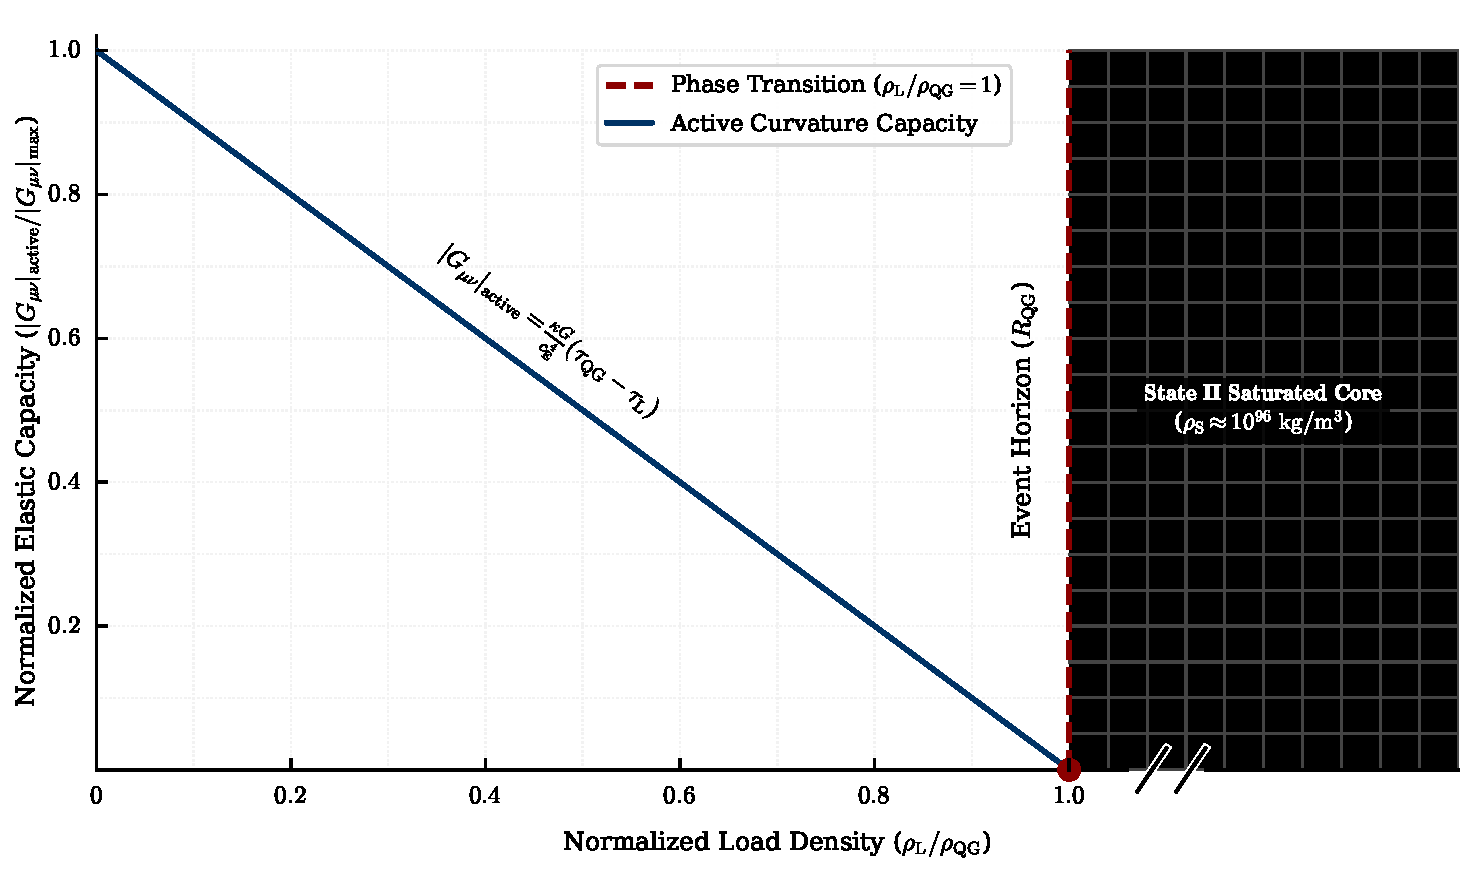
\includegraphics[width=0.9\textwidth]{FigX_PartII_Curvature.pdf}
    \caption{\textbf{The Arrest of Kinematic Curvature.} Normalized active curvature capacity $|G_{\mu\nu}|_{\mathrm{active}} / |G_{\mu\nu}|_{\mathrm{max}}$ as a function of the normalized local mass-energy load density $\rho_{\mathrm{L}} / \rho_{\mathrm{QG}}$. Dictated by the Conservation of Structural Integrity, observable gravity manifests strictly as active lattice strain. In the Soft Floor regime ($\rho_{\mathrm{L}} < \rho_{\mathrm{QG}}$), the available geometric capacity of the elastic vacuum decays linearly as localized baryonic mass saturates the native octahedral interstitial voids of the FCC lattice (see \hyperref[part:three]{Part III}). This capacity deficit is governed by the restorative tension relation $|G_{\mu\nu}|_{\mathrm{active}} = \frac{\kappa G}{c_{\mathrm{E}}^4}(\tau_{\mathrm{QG}} - \tau_{\mathrm{L}})$. At the exact convergence threshold ($\rho_{\mathrm{L}} / \rho_{\mathrm{QG}} = 1.0$), remaining structural elasticity drops identically to zero (maroon node), triggering an instantaneous hyperstatic yield. This boundary marks the Event Horizon ($R_{\mathrm{QG}}$), past which the active metric field terminates. The system abruptly enters the State II Saturated Core ($\rho_{\mathrm{S}} \approx 10^{96}$ kg/m$^3$), visually represented by the broken density axis ($//$) and the structurally phase-locked Simple Cubic (SC) background matrix. Within this rigid core, the saturated region undergoes a geometric phase transition to absolute structural degeneracy ($\Delta\phi = 0$); active kinematic curvature is not mathematically divergent, but mechanically terminated.}
\label{fig:arrest_kinematic_curvature}
\end{figure}

\subsection{The Tensor Projection of the Active Tension Balance}

While the scalar equation governs the magnitude of the interaction, it does not by itself encode directional stress structure. To compare the TFT strain law with standard four-dimensional gravitational bookkeeping, the scalar active-balance relation is projected into an effective tensor-valued form.

In this projection, the isotropic capacity of the active vacuum supplies the background floor, while localized matter-energy supplies the load:
\begin{itemize}
    \item \textbf{The floor:} $\tau_{\mathrm{QG}} \to \tau_{\mathrm{QG}}\eta_{\mu\nu}$, representing the isotropic active background capacity of the unbroken Soft Floor.
    \item \textbf{The load:} $\tau_{\mathrm{L}} \to T_{\mu\nu}$, where the scalar matter-energy load expands into the standard stress-energy tensor of localized mass-energy and radiation.
\end{itemize}

The effective tension-curvature projection is therefore written as:
\begin{equation}
    G_{\mu\nu}^{(\tau)} = \frac{\kappa G}{c_{\mathrm{E}}^4} \left( \tau_{\mathrm{QG}}\eta_{\mu\nu} - T_{\mu\nu} \right).
\end{equation}

Here, $G_{\mu\nu}^{(\tau)}$ should not be interpreted as fundamental curvature of an empty spacetime manifold. It is the effective tensor representation of active lattice strain produced by the difference between the available vacuum tension capacity and the local matter-energy load.

This formulation preserves the directional information needed for comparison with relativistic gravitational phenomenology while maintaining the TFT ontology: gravity is fundamentally a restorative strain and refractive response of the active vacuum, with metric-like curvature appearing only as an effective observational projection.

\subsection{Cosmological Integration: The \texorpdfstring{$\beta \to T_{\mu\nu}$}{beta to T\_mu nu} Mapping}
\label{sec:cosmological_integration}
To satisfy macroscopic cosmological observations, we must explicitly map the geometric packing fractions ($\beta$) derived in Part I to the background stress-energy tensor. 

In standard $\Lambda$CDM cosmology, the macroscopic universe is governed by the energy density parameters ($\Omega$). In Tension Field Theory, because the vacuum is a contiguous elastic medium, the absolute cosmological background capacity is determined by the fundamental structural yield tension of the lattice ($\tau_{\mathrm{G}}$). While the local active field equation is bounded by the scale-dependent convergence capacity ($\tau_{\mathrm{QG}}$) to govern localized phase transitions (Black Holes), the total geometric energy budget of the unbroken universe is dictated by its absolute structural limit ($\tau_{\mathrm{G}}$).

Crucially, we must distinguish between operational inertial density and structural yield capacity. While the solid nodes ($\rho_{\mathrm{D}}$) and the interstitial condensate ($\rho_{\mathrm{IC}}$) possess vastly different operational inertial densities, the macroscopic framework is strictly governed by the universal Gravitational Yield Density ($\rho_{\mathrm{D,G}}$). Because the geometric volume of the interstitial voids is structurally maintained by the exact same hyper-rigid bonds that define the solid nodes, the absolute structural tension capacity ($\tau_{\mathrm{G}} = \rho_{\mathrm{D,G}} c_{\mathrm{E}}^2$) is a uniform macroscopic property. Therefore, this universal background tension is physically partitioned strictly by the spatial volume fractions of the FCC geometry.

Since $\beta_{\mathrm{geo}} + \beta_{\mathrm{IC}} = 1$, we can formally expand the universal active background tensor into its distinct geometric phases:
\begin{equation}
    \tau_{\mathrm{G}} \eta_{\mu\nu} = \tau_{\mathrm{G}} \big( \beta_{\mathrm{geo}} + \beta_{\mathrm{IC}} \big) \eta_{\mu\nu}
\end{equation}

Substituting this partitioned global background into the TFT Tensor Field Equation bridges the microscopic lattice geometry directly to the macroscopic cosmic energy budget:
\begin{equation}
    G_{\mu\nu} = \frac{\kappa G}{c_{\mathrm{E}}^4} \Big( \big[\beta_{\mathrm{geo}} \tau_{\mathrm{G}} \eta_{\mu\nu}\big] + \big[\beta_{\mathrm{IC}} \tau_{\mathrm{G}} \eta_{\mu\nu}\big] - T_{\mu\nu} \Big)
\end{equation}

This expanded tensor rigorously maps to the phenomenological $\Omega$ parameters without requiring exotic particles or negative thermodynamic pressure:
\begin{itemize}
    \item \textbf{The Structural Tensor ($\beta_{\mathrm{geo}} \tau_{\mathrm{G}} \eta_{\mu\nu} \longrightarrow \Omega_{\Lambda}$):} The 74\% FCC solid node fraction provides the non-clustering, hyperstatic structural tension of the vacuum, masquerading observationally as Dark Energy.
    \item \textbf{The Interstitial Tensor ($\beta_{\mathrm{IC}} \tau_{\mathrm{G}} \eta_{\mu\nu} \longrightarrow \Omega_{\mathrm{DM}}$):} The 26\% fluidic void fraction provides the dynamic kinematic impedance, dragging around baryonic defects to masquerade observationally as clustering Dark Matter halos.
    \item \textbf{The Load Tensor ($T_{\mu\nu} \longrightarrow \Omega_{\mathrm{b}}$):} The standard stress-energy tensor represents the localized baryonic vibrational defects actively consuming the background capacity. 
\end{itemize}

When evaluated over macroscopic cosmological scales, this localized load tensor mathematically averages exactly to the $\approx 5\%$ baryonic defect fraction derived in Section 6.5: $\langle T_{\mu\nu} \rangle = \beta_{\mathrm{b}} \tau_{\mathrm{G}} \eta_{\mu\nu}$. Applying this macroscopic cosmic average to the entire field equation ($\langle G_{\mu\nu} \rangle$) reveals that the baryonic load directly subtracts from the solid node capacity:
\begin{equation}
    \langle G_{\mu\nu} \rangle = \frac{\kappa G}{c_{\mathrm{E}}^4} \Big( \big[\beta_{\mathrm{geo}} - \beta_{\mathrm{b}}\big] \tau_{\mathrm{G}} \eta_{\mu\nu} + \big[\beta_{\mathrm{IC}}\big] \tau_{\mathrm{G}} \eta_{\mu\nu} \Big)
\end{equation}

This mechanically proves the reduced effective Dark Energy density ($\beta_{\Lambda,\mathrm{eff}} = \beta_{\mathrm{geo}} - \beta_{\mathrm{b}}$). By projecting the scalar geometric limits ($\beta$) into the background coefficients of the active metric tensor, TFT mathematically recovers the observed cosmological density parameters ($\Omega$) from pure solid-state first principles. \textit{(Note: The mechanical validity of projecting these geometric properties into the standard GR stress-energy tensor is independently verified by dynamic wave propagation; see \hyperref[app:kinematic_shear]{Appendix \ref*{app:kinematic_shear}} for the exact recovery of the spin-2 strain tensor from the macroscopic lattice shear modulus).}

\section{The Optical Analogy: Gravity as a Refractive Medium}
In \hyperref[part:one]{Part I} (\hyperref[postulate:four]{Postulate IV}), we differentiated the invariant energy constant $c_{\mathrm{E}}$ from the dynamic propagation speed $c_{\mathrm{P}}$, where $c_{\mathrm{P}}$ is a variable governed by the local effective inertia $\mu_{\mathrm{eff}}$. In this section, we demonstrate that the metric tensor of General Relativity is functionally identical to the variable refractive index $n$ created by this inertial density.

Furthermore, to address the relationship between the mechanical vacuum and relativistic observations, we distinguish between two distinct regimes of measurement, both fundamentally modulated by the unitary lattice strain $\alpha_{\mathrm{G}}$:
\begin{itemize}
    \item \textbf{Intrinsic physics:} The objective state of the source.
    \item \textbf{Observed physics:} The integration of the wave path.
\end{itemize}

\subsection{The Vacuum as a Variable Dielectric}
\label{sec:refractive_index}

In previous sections, we established that gravity is not a geometric curvature of empty space, but a physical variation in the strain state of the active vacuum lattice. Light, in this framework, is a minimum transverse tension ripple propagating through that strained medium. We now show that the weak-field metric behavior normally attributed to spacetime curvature can be represented mechanically as the refractive index of the active vacuum.

We define the general strain-induced vacuum refractive index $n_\tau(\mathbf{x})$ as the ratio of the invariant lattice kinematic budget $c_{\mathrm{E}}$ to the local propagation speed $c_{\mathrm{P}}$ of a causal signal:
\begin{equation}
    n_\tau(\mathbf{x}) = \frac{c_{\mathrm{E}}}{c_{\mathrm{P}}}.
\end{equation}

Here the spatial argument $\mathbf{x}$ is attached to $n_\tau$, because the refractive index is the field quantity that varies across the strained Soft Floor. The propagation speed $c_{\mathrm{P}}$ is understood as the corresponding local signal speed at the point being considered.

Using the effective optical inertia derived in \hyperref[sec:discrete_state_transfer]{Section \ref*{sec:discrete_state_transfer}}, where
\begin{equation}
    \mu_{\mathrm{eff}} \propto (1-\alpha_{\mathrm{G}})^{-4},
\end{equation}
the local propagation speed of a transverse signal through the strained Soft Floor is
\begin{equation}
    c_{\mathrm{P}} = c_{\mathrm{E}} (1-\alpha_{\mathrm{G}})^2.
\end{equation}

Therefore, the general strain-induced refractive index is
\begin{equation}
    n_\tau(\mathbf{x}) = \frac{1}{(1-\alpha_{\mathrm{G}})^2}.
\end{equation}

In this expression, $\alpha_{\mathrm{G}}$ denotes the local value of the gravitational strain variable at the point $\mathbf{x}$. When no ambiguity arises, its spatial argument is suppressed for compactness.

For a static, spherically symmetric source of mass $M$, the local strain variable reduces to
\begin{equation}
    \alpha_{\mathrm{G}} = \frac{GM}{rc_{\mathrm{E}}^2}.
\end{equation}

In that special spherical case, the refractive index becomes
\begin{equation}
    n_\tau(r) = \frac{c_{\mathrm{E}}}{c_{\mathrm{P}}} = \frac{1}{(1-\alpha_{\mathrm{G}})^2}.
\end{equation}

In the weak-field limit, where
\begin{equation}
    \alpha_{\mathrm{G}} \ll 1,
\end{equation}
we apply the binomial approximation
\begin{equation}
    (1-x)^{-2} \approx 1+2x.
\end{equation}

Thus,
\begin{equation}
    n_\tau(r) \approx 1+2\alpha_{\mathrm{G}} = 1+\frac{2GM}{rc_{\mathrm{E}}^2}.
\end{equation}

This result shows that the weak-field optical correction normally encoded by the spatial part of the General Relativistic metric can be reinterpreted mechanically as the refractive response of the active vacuum lattice. In TFT, the apparent curvature experienced by light is therefore not fundamental curvature of empty spacetime, but the optical consequence of strain-induced propagation through the Soft Floor.

\subsection*{The Mechanics of Time Dilation ($1\alpha_{\mathrm{G}}$)}

We must distinguish between the intrinsic state of a system and the observed measurement of that system. This distinction resolves the confusion between local time dilation and remote signal delay.

\vspace{0.5em}
\noindent\textbf{The Intrinsic State:}\\
In \hyperref[postulate:two]{Postulate II}, we established that for localized mass, Proper Time ($t_{\mathrm{p}}$) is the emergent internal clock defined strictly by the accumulation of stationary, integer $360^{\circ}$ volumetric phase cycles ($n$). The duration of a single phase cycle (one fundamental ``tick'') is governed by the structural energy coupling: $t_{\mathrm{tick}} = h/E$.

\vspace{0.5em}
\noindent\textbf{Phase Damping (The Strain Deficit):}\\
In Tension Field Theory, an atomic clock functions as a harmonic oscillator coupled to the lattice. In a region of high macroscopic lattice strain ($\alpha_{\mathrm{G}}$), a fraction of the vacuum's baseline elastic capacity is pre-emptively consumed by the gravitational tension. Consequently, the local rest energy ($E_{\alpha}$) available to drive the node's rotation is proportionally reduced relative to the unstrained vacuum baseline ($E_0$):
\begin{equation}
    E_{\alpha} = E_0(1 - \alpha_{\mathrm{G}})
\end{equation}

Because the physical energy driving the rotation is damped, the node struggles against the visco-elastic damping of the medium and physically takes longer to complete a single $2\pi$ phase cycle. The expanded duration of Proper Time on the strained surface ($t_{\mathrm{p}, \alpha}$) relative to the unstrained vacuum baseline ($t_{\mathrm{p}, 0}$) becomes:
\begin{equation}
    t_{\mathrm{p}, \alpha} = n \left( \frac{h}{E_0(1 - \alpha_{\mathrm{G}})} \right) = \frac{t_{\mathrm{p}, 0}}{1 - \alpha_{\mathrm{G}}}
\end{equation}

\vspace{0.5em}
\noindent\textbf{Conclusion:}\\
The apparent slowing of time is not a geometric curvature of a background temporal dimension, but a strict mechanical consequence of Phase Damping. The ($\alpha_{\mathrm{G}}$) local energy deficit physically forces the fundamental structural clock to rotate more slowly. When this damped node emits a wave, the sequential phase transfer is inherited by the emission, matching gravitational redshift observations exactly without invoking geometric curvature.

\vspace{0.5em}
\noindent\textbf{Corollary: Gravitational Length Contraction (Structural Sag)}\\
Just as Phase Damping slows the internal clock of a localized mass, it also physically deforms its spatial footprint. A macroscopic object is held together by internal structural bonds (transverse shear waves). Because the local elastic capacity is pre-emptively consumed by gravitational tension ($\alpha_{\mathrm{G}}$), the available energy to maintain these bonds drops to $E_{\alpha} = E_0(1 - \alpha_{\mathrm{G}})$. Lacking the full baseline energy to hold the constituent atoms apart, the object's structural bonds physically compress to reach mechanical equilibrium with the surrounding vacuum. Therefore, while the underlying geometric lattice ($r_{\mathrm{D}}$) remains invariant, the macroscopic object itself physically shrinks in the direction of the tension gradient by the exact ratio of the strain deficit: $L_{\alpha} = L_0 (1 - \alpha_{\mathrm{G}})$.

\subsection{From Strain-Weighted Paths to the Effective Optical Metric}
\label{sec:optical_metric}
The strain-weighted path functional introduced in Part I defines the accumulated spatial penalty experienced by a propagating excitation moving through a nonuniform tension field. At the postulate level, this object is written compactly as
\begin{equation}
    D_\tau = \int \left( 1 + \frac{r_{\mathrm{D}}}{\tau_{\mathrm{S}}} |\nabla\tau(\mathbf{x})| \right) \mathrm{d}\ell .
\end{equation}
This expression is not a spacetime metric tensor. It is a scalar path functional: it measures the accumulated spatial cost of propagation through the active vacuum. When the path dependence must be made explicit, we write
\begin{equation}
    D_\tau[\mathcal{P}] = \int_{\mathcal{P}} n_\tau(\mathbf{x}) \, \mathrm{d}\ell ,
\end{equation}
where $\mathcal{P}$ denotes the chosen propagation path and $n_\tau(\mathbf{x})$ is the local strain-induced optical index of the active vacuum.

In the gravitational optical limit developed above, this strain index is governed by the local gravitational coupling
\begin{equation}
    \alpha_{\mathrm{G}} = \frac{GM}{rc_{\mathrm{E}}^2}.
\end{equation}
Since the dynamic propagation speed of a transverse signal through the strained Soft Floor is
\begin{equation}
    c_{\mathrm{P}} = c_{\mathrm{E}}(1-\alpha_{\mathrm{G}})^2,
\end{equation}
the corresponding effective refractive index is
\begin{equation}
    n_\tau(r) = \frac{c_{\mathrm{E}}}{c_{\mathrm{P}}(r)} = \frac{1}{(1-\alpha_{\mathrm{G}})^2}.
\end{equation}
Thus, in the gravitational propagation regime, the path functional becomes
\begin{equation}
    D_\tau[\mathcal{P}] = \int_{\mathcal{P}} \frac{1}{(1-\alpha_{\mathrm{G}})^2} \, \mathrm{d}\ell .
\end{equation}
The corresponding optical travel time is
\begin{equation}
    \Delta t = \frac{1}{c_{\mathrm{E}}} \int_{\mathcal{P}} n_\tau(\mathbf{x}) \, \mathrm{d}\ell = \frac{1}{c_{\mathrm{E}}} \int_{\mathcal{P}} \frac{1}{(1-\alpha_{\mathrm{G}})^2} \, \mathrm{d}\ell .
\end{equation}
The physical path followed by a freely propagating light signal is therefore obtained by the least-time condition
\begin{equation}
    \delta \int_{\mathcal{P}} n_\tau(\mathbf{x}) \, \mathrm{d}\ell = 0.
\end{equation}
This is the TFT refractive form of the null-path condition. It does not require fundamental curvature of an empty manifold. Instead, the apparent bending of light arises because the wave follows the path of stationary optical time through the strain-index field of the active vacuum.

To compare this refractive mechanics with the standard language of General Relativity, we may package the same propagation law into an effective Soft Floor measurement tensor. For a static, isotropic gravitational strain field, the minimal operational line element is
\begin{equation}
    \mathrm{d}s_\tau^2 = -(1-\alpha_{\mathrm{G}})^2 c_{\mathrm{E}}^2 \mathrm{d}t^2 + (1-\alpha_{\mathrm{G}})^{-2} \delta_{ij} \mathrm{d}x^i \mathrm{d}x^j .
\end{equation}
This defines the effective metric tensor
\begin{equation}
    g_{\mu\nu}^{(\tau)} = \mathrm{diag} \left[ -(1-\alpha_{\mathrm{G}})^2 c_{\mathrm{E}}^2, (1-\alpha_{\mathrm{G}})^{-2}, (1-\alpha_{\mathrm{G}})^{-2}, (1-\alpha_{\mathrm{G}})^{-2} \right]
\end{equation}
in locally isotropic spatial coordinates.

For a null path,
\begin{equation}
    \mathrm{d}s_\tau^2 = 0.
\end{equation}
Therefore,
\begin{equation}
    (1-\alpha_{\mathrm{G}})^2 c_{\mathrm{E}}^2 \mathrm{d}t^2 = (1-\alpha_{\mathrm{G}})^{-2} \mathrm{d}\ell^2,
\end{equation}
which gives
\begin{equation}
    \frac{\mathrm{d}\ell}{\mathrm{d}t} = c_{\mathrm{E}}(1-\alpha_{\mathrm{G}})^2 = c_{\mathrm{P}}.
\end{equation}
Thus the effective metric reproduces exactly the TFT propagation law for light through the strained Soft Floor.

In the weak-field limit, where
\begin{equation}
    \alpha_{\mathrm{G}} \ll 1,
\end{equation}
we have
\begin{equation}
    (1-\alpha_{\mathrm{G}})^2 \approx 1-2\alpha_{\mathrm{G}},
\end{equation}
and
\begin{equation}
    (1-\alpha_{\mathrm{G}})^{-2} \approx 1+2\alpha_{\mathrm{G}}.
\end{equation}
The effective line element therefore becomes
\begin{equation}
    \mathrm{d}s_\tau^2 \approx -(1-2\alpha_{\mathrm{G}}) c_{\mathrm{E}}^2 \mathrm{d}t^2 + (1+2\alpha_{\mathrm{G}}) \mathrm{d}\ell^2 .
\end{equation}
Using the Newtonian potential
\begin{equation}
    \Phi = -\frac{GM}{r},
\end{equation}
so that
\begin{equation}
    \alpha_{\mathrm{G}} = -\frac{\Phi}{c_{\mathrm{E}}^2},
\end{equation}
the weak-field expression becomes
\begin{equation}
    \mathrm{d}s_\tau^2 \approx -\left( 1+\frac{2\Phi}{c_{\mathrm{E}}^2} \right) c_{\mathrm{E}}^2 \mathrm{d}t^2 + \left( 1-\frac{2\Phi}{c_{\mathrm{E}}^2} \right) \mathrm{d}\ell^2 .
\end{equation}
This is the standard weak-field relativistic form, recovered here as an effective optical geometry of the active vacuum. In this limit, TFT reproduces the operational metric behavior associated with gravitational redshift, Shapiro delay, and weak-field light deflection (Note: Massive bound orbits probe a different channel of the same strained Soft Floor: the conservative coupling between radial strain potential and tangential topological transport. The corresponding perihelion precession mechanism is introduced in \hyperref[sec:perihelion_strain_coupling]{Section~\ref*{sec:perihelion_strain_coupling}} and derived fully in \hyperref[app:perihelion_orbital_strain]{Appendix~\ref*{app:perihelion_orbital_strain}}).

The tensor $g_{\mu\nu}^{(\tau)}$ should therefore be read as an effective Soft Floor measurement tensor. Under coordinate relabeling, it transforms as a tensor,
\begin{equation}
    g_{\alpha\beta}^{(\tau)\prime} = \frac{\partial x^\mu}{\partial x^{\prime\alpha}} \frac{\partial x^\nu}{\partial x^{\prime\beta}} g_{\mu\nu}^{(\tau)}.
\end{equation}
If desired, one may construct the corresponding connection and curvature objects from $g_{\mu\nu}^{(\tau)}$ using the standard differential-geometric machinery. However, in TFT these objects are not fundamental causes of gravity. They are the observational bookkeeping of a deeper mechanical process: localized matter-energy changes the strain state of the active vacuum, the strain field changes the local refractive index, and the refractive index determines the effective paths of waves, rods, and clocks.

Therefore, TFT does not treat spacetime curvature as the fundamental origin of gravity. Rather, curvature appears as the effective geometric representation of strain-induced refractive propagation through the Soft Floor.
The same strain variable $\alpha_{\mathrm{G}}$ that generates the weak-field optical metric also defines the nonlinear failure boundary of the active vacuum. In the weak-field regime ($\alpha_{\mathrm{G}} \ll 1$), TFT reproduces the operational metric behavior of General Relativity. In the saturation regime ($\alpha_{\mathrm{G}} \to 1$), however, TFT does not extend the effective metric to a geometric singularity. Instead, the active FCC Soft Floor reaches its finite mechanical yield limit and undergoes a phase transition into the phase-locked SC Substrate. Thus, the GR singularity is replaced by a physical lattice-saturation boundary.

\subsection{The Mechanics of Light Propagation ($2\alpha_{\mathrm{G}}$)}
\label{sec:lightspeed_mechanics}
While a stationary clock only suffers from the localized energy deficit ($1\alpha_{\mathrm{G}}$), a propagating signal such as a radar ping interacts dynamically with the strained vacuum medium across space.
\vspace{0.5em}

\noindent \textbf{The Variable Speed of Light ($c_{\mathrm{P}}$):} Due to the transverse nature of electromagnetic waves, the optical inertia scales quadratically with the lattice strain, $\mu_{\mathrm{eff}} \propto (1 - \alpha_{\mathrm{G}})^{-4}$. This imposes a double penalty on the traversing wave derived from the medium itself:
\begin{itemize}
    \item \textbf{Temporal Impedance ($1\alpha_{\mathrm{G}}$):} Caused by the reduced vibrational rate of the local vacuum nodes. Because the strained medium oscillates more slowly under the local energy deficit, the sequential transmission of the wave is mechanically delayed.
    \item \textbf{Spatial Impedance ($1\alpha_{\mathrm{G}}$):} Caused by the physical deformation of the lattice, requiring the wave to traverse spatially stretched node geometries.
\end{itemize}

As derived earlier, the effective strain-induced refractive index is
\begin{equation}
    n_\tau(r) \approx 1 + 2\alpha_{\mathrm{G}}.
\end{equation}
Consequently, the local propagation speed of light is not a fixed coordinate speed, but a variable determined by the local strain state of the active vacuum:
\begin{equation}
    c_{\mathrm{P}}(r) = \frac{c_{\mathrm{E}}}{n_\tau(r)} \approx c_{\mathrm{E}}(1 - 2\alpha_{\mathrm{G}}).
\end{equation}

Because the signal travels more slowly than the unstrained vacuum baseline ($c_{\mathrm{P}} < c_{\mathrm{E}}$), it accumulates a time delay when traversing a gravitational potential. The total flight time $\Delta t$ is obtained by integrating the inverse propagation speed along the geometric path:
\begin{equation}
    \Delta t = \int \frac{1}{c_{\mathrm{P}}} \, \mathrm{d}\ell = \int \frac{n_\tau(r)}{c_{\mathrm{E}}} \, \mathrm{d}\ell \approx \frac{1}{c_{\mathrm{E}}} \int (1 + 2\alpha_{\mathrm{G}}) \, \mathrm{d}\ell .
\end{equation}

\noindent\textbf{Conclusion:} The factor of $2\alpha_{\mathrm{G}}$ accounts for the Shapiro delay \cite{Shapiro_1964}. \textit{(The full step-by-step macroscopic integration recovering the logarithmic delay is provided in \hyperref[app:optical_relativity]{Appendix~\ref*{app:optical_relativity}})}. This confirms that the mechanics of light propagation rely on a variable local propagation speed, and that the observed time delay is the integral of this reduced velocity through a strain-induced refractive medium.
\vspace{0.5em}

\noindent \textbf{The Artifact of Local Invariance:}
While $c_{\mathrm{P}}$ objectively decelerates relative to the absolute vacuum baseline ($c_{\mathrm{E}}$) by a factor of $2\alpha_{\mathrm{G}}$, a local observer situated within the gravitational potential cannot detect this deceleration. This is governed by strict kinematic coupling:
\begin{itemize}
    \item Both the propagating signal (light) and the physical tools measuring it (matter) are mechanical excitations of the exact same FCC lattice nodes.
    \item Consequently, the observer's measurement tools suffer the exact same refractive strain ($\alpha_{\mathrm{G}}$) as the light wave itself.
    \item \textbf{The Covariant Cancellation:} The local atomic clock is damped by the $1\alpha_{\mathrm{G}}$ energy deficit, causing it to tick slower (Time Dilation). Simultaneously, the structural bonds of the observer's ruler are weakened by the same $1\alpha_{\mathrm{G}}$ deficit, causing the physical object to compress (Length Contraction).
\end{itemize}

When an observer uses a proportionally shrunken ruler to measure distance ($D_{\mathrm{obs}} = D_{\mathrm{true}}/(1 - \alpha_{\mathrm{G}})$) and a proportionally slowed clock to measure time ($T_{\mathrm{obs}} = T_{\mathrm{true}}\cdot(1 - \alpha_{\mathrm{G}})$), dividing distance by time ($D/T$) yields a combined measurement handicap of
\begin{equation}
    \frac{1}{(1-\alpha_{\mathrm{G}})^2} \approx 1 + 2\alpha_{\mathrm{G}}.
\end{equation}

This handicap mathematically cancels the signal's $2\alpha_{\mathrm{G}}$ deceleration. Therefore, the locally measured invariance of $c$ in General Relativity is reinterpreted in TFT as a localized measurement artifact---the inevitable mathematical consequence of conducting kinematics inside a covariant refractive medium using tools made of that same medium.

\subsection{Gravitational Lensing ($4\alpha_{\mathrm{G}}$)}
The most famous prediction of relativity---the bending of starlight---is a direct consequence of the refractive gradient. Light follows the stationary optical-time path through a spherical strain-index field. The explicit evaluation of the transverse refractive gradient, yielding the total deflection angle of $4\alpha_{\mathrm{G}}(b)$, is detailed in \hyperref[app:optical_relativity]{Appendix~\ref*{app:optical_relativity}}.

Consider a wavefront passing a massive object at an impact parameter $b$. The inner part of the wavefront, closer to the mass, travels through a region of higher refractive index ($n_{\tau, \mathrm{high}}$) and thus moves more slowly than the outer part ($n_{\tau, \mathrm{low}}$). This velocity differential causes the wavefront to steer toward the mass.

The total deflection angle $\theta$ is the magnitude of the accumulated transverse refractive-gradient steering along the full line-of-sight path $z$. Let $b$ be the impact parameter---the perpendicular distance from the center of mass to the unperturbed photon path---such that the radial distance is
\begin{equation}
    r = \sqrt{b^2 + z^2}.
\end{equation}

The deflection magnitude is therefore
\begin{equation}
    \theta = \left| \int_{-\infty}^{+\infty} \nabla_{\perp} n_\tau \, \mathrm{d}z \right| = \left| \int_{-\infty}^{+\infty} \frac{\partial}{\partial b} \left( 1+ \frac{2GM}{c_{\mathrm{E}}^2\sqrt{b^2 + z^2}} \right) \mathrm{d}z \right|.
\end{equation}

The integration accumulates the transverse refractive steering along the geometric path, yielding
\begin{equation}
    \theta_{\mathrm{total}} = \frac{4GM}{b c_{\mathrm{E}}^2} = 4\alpha_{\mathrm{G}}(b).
\end{equation}

\noindent\textbf{Conclusion:} Tension Field Theory recovers the precise Einstein deflection angle, approximately $1.75$ arcseconds for the Sun, purely through wave optics.

The factor of $4$ arises from integrating the transverse gradient of the weak-field refractive index
\begin{equation}
    n_\tau(r) \approx 1 + 2\alpha_{\mathrm{G}}(r)
\end{equation}
along the full line-of-sight path. Furthermore, this macroscopic factor of $4$ is interpreted in TFT as the geometric signature of the photon wave packet being compressed across the four degrees of freedom of the FCC lattice: longitudinal, temporal, and two transverse. As demonstrated in \hyperref[part:three]{Part III} (\hyperref[sec:photonic_relaxation]{Section~\ref*{sec:photonic_relaxation}}), this exact four-dimensional optical impedance acts as the mechanical mirror to the Tolman surface brightness drop \cite{Tolman_1930}, where the wave packet isotropically relaxes across those same four dimensions to yield a $(1+z)^{-4}$ reduction in apparent optical power.

\begin{table}[H]
\centering
\caption{\textbf{Summary of Relativistic Coefficients}}
\label{tab:relativistic_coefficients}
\renewcommand{\arraystretch}{1.5}
\begin{tabular}{@{}llc@{}}
\toprule
\textbf{Phenomenon} & \textbf{TFT Mechanism} & \textbf{Coefficient} \\
\midrule
Gravitational redshift & Mechanical damping (source energy deficit) & $1\alpha_{\mathrm{G}}$ \\
Shapiro delay & Optical refraction (path impedance) & $2\alpha_{\mathrm{G}}$ \\
Light deflection & Gradient steering (integrated refraction) & $4\alpha_{\mathrm{G}}(b)$ \\
\bottomrule
\end{tabular}
\end{table}